% Kapitel 'Grundlagen der 3D-Grafik'
\chapter{Grundlagen der 3D-Grafik}
\label{grafikgrundlagen}

Ging es im vorigen Kapitel um die nötigen mathematischen Konzepte, werde ich versuchen, in den folgenden Abschnitten einen Überblick über die Umsetzung der 3D-Grafik am Computer zu geben, bevor wir uns in Kapitel \ref{3d-transformations} und \ref{viewingtransformations} genauer mit den dafür nötigen mathematischen Operationen und Algorithmen beschäftigen werden.

Rufen wir uns zunächst einmal das Ziel der 3D-Grafik in Erinnerung: das Erzeugen eines zweidimensionalen Bildes aus einer Beschreibung einer dreidimensionalen Umgebung (Szene). Daraus ergibt sich mehr oder weniger von selbst eine Unterteilung in zwei Bereiche, nämlich die digitale Repräsentation einer Szene, der sogenannten \emph{Modellierung}, und die eigentlichen Berechnung des Bildes, der \emph{Bildsynthese} (viel gebräuchlicher ist der englische Begriff \emph{Rendering}).

Die Modellierung erfolgt in der Regel manuell (wenn man von Experimenten etwa mit fraktaler Geometrie absieht) und kann auf vielfältige Weisen geschehen, zum Beispiel durch Digitalisierung von realen Gegenständen durch einen 3D-Scanner oder durch händische Erstellung des Modelles mittels Modellierungssoftware am Computer. Diese vorbereiteten Daten sind die Ausgangsbasis für das Rendering, das dann automatisch abläuft.

Grundsätzlich ist zwischen zwei großen Einsatzbereichen der 3D-Grafik zu unterscheiden. Der eine ist die unmittelbar durch den Benutzer gesteuerte Erzeugung von Ansichten einer 3D-Szene in Echtzeit, zum Beispiel in einem Computerspiel oder einem CAD-Programm. Der andere ist die Berechnung mehr oder weniger realistischer Bilder, beispielsweise in einem Animationsfilm oder zur Architekturvisualisierung.

Den beiden Einsatzbereichen gemein ist die stete Forderung nach Effizienz. Bei der interaktiven Anwendung muss eine gewisse Anzahl an Bilder pro Zeitintervall (typischerweise 20-30 Bilder pro Sekunde) mit einer begrenzten Rechenleistung erzeugt werden, damit die Darstellung für das Auge flüssig wirkt und die Eingaben des Benutzers ohne merkbare Verzögerung umgesetzt werden. Bei der Berechnung eines realistischen Bildes wird zwar im Normalfall viel mehr Rechenaufwand pro Bild akzeptiert, aber auch hier wird versucht, die benötigte Zeit möglichst gering zu halten, da so Korrekturen leichter möglich sind, aber auch schlicht der Aufwand und somit die Kosten sinken.

Deswegen wird immer nach Verfahren gesucht, die mit möglichst geringem Rechenaufwand und Speicherplatzbedarf die Ergebnisse aufwändiger Berechnungen möglichst gut annähern. Diese Verfahren müssen mit den realen Phänomen nicht mehr unbedingt viel zu tun haben, so lange das Ergebnis echt genug erscheint, um das Auge zu täuschen.

Die in diesem Kapitel geschilderten Grundlagen sind in einschlägiger Fachliteratur nachzulesen, im Besonderen seien die im Anhang \enquote{\bibname} gelisteten Werke \enquote{3D-Spiele mit C++ und DirectX} \citep{21tage} und \enquote{3D-Spiele-Programmierung} \citep{kompendium} erwähnt.


\section{Modellierung}
Wie schon erwähnt, ist das Ziel der Modellierungsphase, eine digitale Repräsentation von (dreidimensionalen) Objekten zu erstellen, anhand welcher später ein Bild berechnet werden kann.
% Szene: Dazu gehören im Wesentlichen die Objekte mit ihren Materialeigenschaften und die Lichtquellen, die die Szene beleuchten.

Hier stößt man schnell auf das Problem, dass die realen phyikalischen Phänomene, die das Erscheinungsbild eines Objektes verursachen, viel zu komplex sind, um exakt nachgebildet werden zu können, vor allem im Hinblick auf die begrenzte Rechenleistung, mit der anschließend die Abbildung erzeugt wird.

Das derzeit am weitesten verbreitete Verfahren, um dieser Komplexität Herr zu werden, beruht darauf, die Speicherung der Form des Objektes (also der Oberfläche) von der des Materials (also der Eigenschaften dieser Oberfläche) zu trennen. Dieses Verfahren, das als \emph{Oberflächendarstellung} (engl. \emph{Boundary Representation}) bezeichnet wird, geht allerdings davon aus, dass die Szene aus Objekten besteht, die eine definierte Oberfläche haben. Manche Dinge, insbesondere atmosphärische Erscheinungen wie Wolken, Nebel, etc. sind daher schwer darzustellen.

Außerdem liefern manche Verfahren ihre Ergebnisse prinzipbedingt in der Form eines \emph{Voxelgitters}\footnote{Voxel: Kofferwort aus \enquote{Volumen} und \enquote{Pixel}, bezeichnet analog zum zweidimensionalen Pixel ein Element eines regelmäßigen dreidimensionalen Gitters.}, also eines dreidimensionales Gitters, bei dem jedem Element ein Wert zugeordnet ist. Dazu zählen unter anderem viele bildgebende Verfahren wie Computertomographie, die in der Forschung und der Medizin verwendet werden. Diese Daten lassen sich naturgemäß leichter mit den Mitteln der \emph{Voxelgrafik} darstellen\footnote{Voxelgrafik bietet noch einige andere Vorteile, wenn es um die Berechnung von fotorealistischen Grafiken geht. So muss man die Zahl der Dreiecke sehr stark erhöhen, wenn man mit den Mitteln der Dreiecksgrafik sehr feine geometrische Strukturen darstellen will. Neben den damit verbundenen Leistungseinbußsen treten einige störende Phänomene wie Flimmern auf, wenn ein großer Teil der Dreiecke am Bildschirm kleiner als ein Pixel ist. Da Voxelgrafik diese Probleme umgeht und für detailreiche Szenen nützliche Optimierungsansätze ermöglicht, wird seit kurzem wieder verstärkt damit experimentiert. \vglr{voxelgraphics}}.

\subsection{Geometrie}
\label{vertex}
Um die Frage zu klären, wie die Oberflächen am effizientesten beschrieben werden können, muss man wissen, wie diese Daten nachher weiterverarbeitet werden, im Falle der 3D-Grafik also gerendert werden -- grundsätzlich sind nämlich viele Varianten denkbar. Die folgenden Aussagen bezüglich Geschwindigkeit gehen von der derzeit in der Echtzeit-3D-Grafik eingesetzen Technik aus, die im Weiteren besprochen wird. Für andere spezielle Rendering-Techniken können sich andere Repräsentationen als effizienter erweisen.

Ein Teil der Verfahren beruht direkt auf einem mathematischen Zusammenhang, zum Beispiel könnte man die Oberfläche einer Kugel (mit dem Mittelpunkt im Koordinatenursprung und dem Radius~$r$) mit Hilfe der Gleichung $x^2 + y^2 + z^2 = r^2$ beschreiben. Sich nur auf mathematische Grundkörper zu beschränken, wäre für die Modellierung realistischer Objekte natürlich viel zu unflexibel, aber es beruhen auch viele andere Verfahren auf Beschreibungen in Gleichungsform. Ein im CAD-Bereich oft eingesetztes Verfahren ist beispielsweise die Darstellung als Rotationskörper einer Polynom- oder einer ähnlichen Funktion\footnote{Polynomfunktionen haben den Nachteil, dass sie bei höherer Ordnung schnell störend schwingen (Runges Phänomen). Abhilfe schaffen andere Interpolationsverfahren wie \emph{Splines}. \vgls{matlab}{73}}.
% Raymarching, prozedurale Geometrie

Diese Darstellungen erlauben zwar eine mathematisch exakte Nachbildung vieler verschiedener Oberflächen -- auch gekrümmte Oberflächen können später aus diesen Daten in beliebiger Genaugkeit bereichnet werden --, aber sie haben gemein, dass die Berechnungen, um aus ihnen Bilder zu erzeugen, für Echtzeitanwendungen (noch) zu aufwändig sind.

Stattdessen wird auf ein wesentlich einfacheres Verfahren zurückgegriffen, nämlich die Darstellung als \emph{Polygonnetz}. Die Oberfläche eines Objektes wird also durch Eckpunkte definiert, die jeweils zu einem Polygon gehören. Diese Punkte werden auch als als \emph{Vertex} (pl. \emph{Vertices}) bezeichnet. Jeder Vertex umfasst zumindest einen Ortsvektor, der seine Position im Raum angibt. Wie in den nächsten Abschnitten erläutert, können einem Vertex aber durchaus noch mehr Daten zugeordnet sein.

\begin{wrapfigure}{R}{0.4\textwidth}
  \vspace{-10pt}
  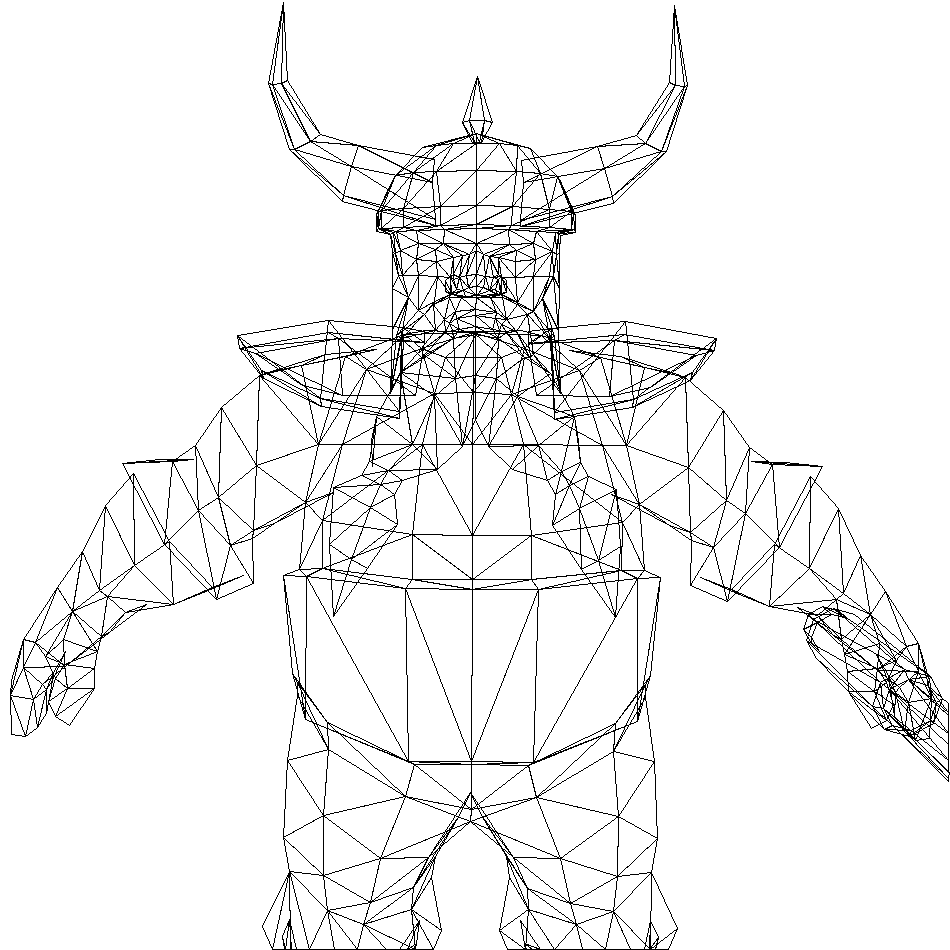
\includegraphics[width=0.39\textwidth]{dwarf_wireframe}
  \vspace{-10pt}
  \caption{Modell eines Zwerges in Wireframe-Darstellung (nur Vorderseiten).}
\end{wrapfigure}

Meist werden nur Polygone mit drei Eckpunkten, also \emph{Dreiecke} verwendet, da sich für diesen Sonderfall viele Algorithmen zur Bildberechnung stark vereinfachen lassen (beispielsweise ist ein Dreieck nie konkav, wodurch sich das Füllen der Bereiche am Bildschirm stark vereinfacht).

Das Polygonnetz kann sowohl direkt in einem entsprechenden Modellierungsprogramm erzeugt werden, als auch aus anderen Darstellungen (zum Beispiel den oben angesprochenen) errechnet werden.

Das Ergebnis kann bereits als so gennantes \emph{Drahtgittermodell} angezeigt werden, auf Englisch wird diese Darstellungsart \emph{Wireframe} genannt. Dabei werden die Vertices einfach durch Linien miteinander verbunden.

\subsection{Oberflächeneigenschaften}
Strenggenommen könnten die Flächen des Modells bereits jetzt gefüllt dargestellt werden. Es fehlen allerdings noch jegliche Informationen über das Material des Objekts. Für die Berechnung eines Bildes sind natürlich in erster Linie die \emph{Reflexionseigenschaften} des Objektes interessant, ist es doch das reflektierte Licht, welches das Bild entstehen lässt.

In der Materialdefinition der Objekte werden daher Informationen über das für das Material typische Reflexionsverhalten gespeichert. Diese Parameter beeinflussen zum Beispiel das Aussehen der Glanzlichter -- auf einer polierten Metallkugel ist die direkte (spekulare) Reflektion der Lichtquelle deutlich abgegrenzt zu erkennen, während eine rauhe Plastikkugel hauptsächlich diffuse Reflexionen zeigen wird. Daneben sind noch einige andere Parameter für Spezialeffekte denkbar, etwa für sogenannte selbstleuchtende Materialien, die auch in der Dunkelheit sichtbar sind.

\begin{wrapfigure}{R}{0.4\textwidth}
  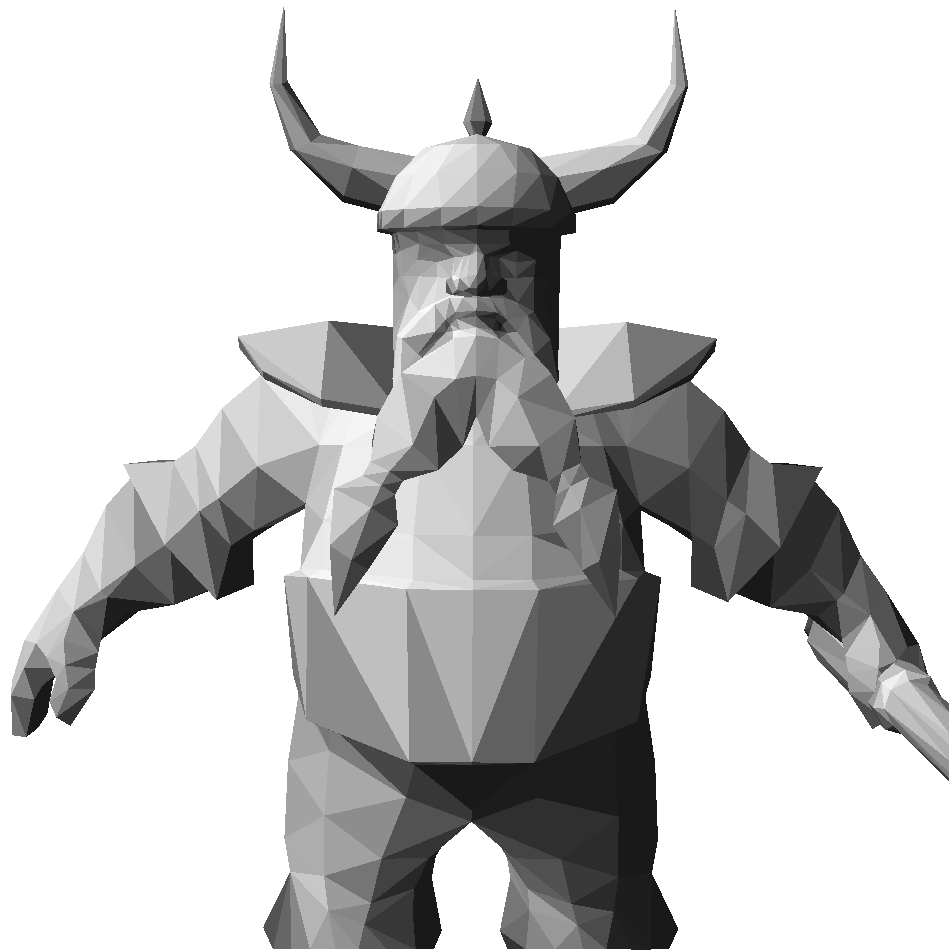
\includegraphics[width=0.39\textwidth]{dwarf_flat}
  \vspace{-10pt}
  \caption{Flat Shading.}
  \label{image:modelflat}
\end{wrapfigure}

Zusätzlich werden jedem Vertex zwei Eigenschaften zugeordnet: die \emph{Farbe} des Eckpunkts und sein \emph{Normalvektor}. Aus diesen Werten, den genannten Materialeigenschaften und den Informationen über die in der Szene vorhandenen Lichtquellen wird der Farbwert des Dreiecks an bestimmten Stellen (und damit der Pixel, die von dem Dreieck abgedeckt werden) berechnet (genaueres in Abschnitt \ref{lighting}).

\label{vertexnormals}
Mittlerweile sollte sich das mathematische Unterbewusstsein schon zu Wort gemeldet haben -- auf einen Vertex, also einen 
% Lz: einem
einzelnen Ortsvektor, lässt sich natürlich keine Normale bilden. Der Grund für diese seltsame Konstruktion liegt in der Verwendung der Normalvektoren für die Lichtberechnung. Zunächst würde man annehmen, dass die Normalvektoren der Eckpunkte eines Polygons ohnehin in die gleiche Richtung zeigen würden. Dies ist grundsätzlich richtig, und mit einer Normale pro Dreieck kann man die Lichtberechnungen auch schon ausführen. Diese Berechnungsart wird als \emph{Flat Shading} bezeichnet.

Der Nachteil dieser Methode wird deutlich, wenn man bedenkt, dass ja aus Effizienzgründen auch alle runden Körper mit Dreiecksnetz angenähert werden. Bei Verwendung von Flat Shading ergeben sich dann hässliche Kanten zwischen den Flächen, wie in Abbildung \ref{image:modelflat} zu sehen.

\begin{wrapfigure}{R}{0.4\textwidth}
  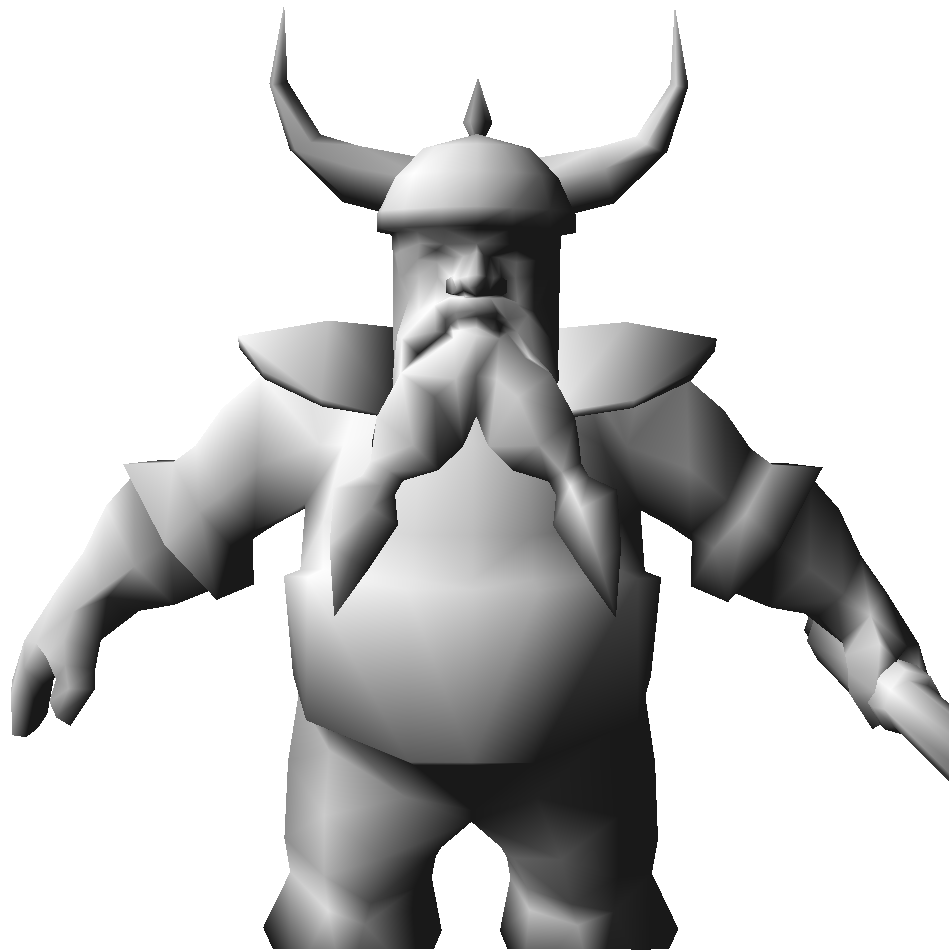
\includegraphics[width=0.39\textwidth]{dwarf_gouraud}
  \vspace{-10pt}
  \caption{Gouraud Shading.}
  \label{image:modelgouraud}	
\end{wrapfigure}

Um dieses Problem zu umgehen, wird nun jedem Vertex ein Normalvektor zugeordnet. Für harte Kanten entspricht dieser weiterhin der Flächennormalen des Dreiecks. Für weiche Kanten hingegen wird dieser Vektor als Mittelwert der Normalvektoren aller angenzenden Flächen berechnet\footnote{Die Interpolation der Normalvektoren aus denen der angrenzenden Flächen ist die einfachste Möglichkeit. Natürlich können die Normalvektoren der Vertices auch anders generiert werden, beispielsweise von Hand durch den Künstler.}. Bei der Helligkeitsberechnung der Pixel, die zu diesem Dreieck gehören, wird dann linear zwischen den Helligkeitswerten der Eckpunkte (\emph{Gouraud Shading}, Abbildung \ref{image:modelgouraud}) oder gleich deren Normalvektoren (\emph{Phong Shading}) interpoliert.

Eine weitere wichtige Materialeigenschaft ist die Transparenz. Dazu ist noch anzumerken, dass eine physikalisch korrekte Simulation der Lichtbrechung und der dadurch hervorgerufenen Phänomene für Echtzeitanwendungen viel zu rechenaufwändig wäre. Statdessen wird im Normalfall das Objekt einfach durchsichtig gezeichnet, die Farbe des dahinter befindlichen Objekts also nicht vollständig überdeckt.

\subsection{Texturen}
\label{texturing}
Bis jetzt sind alle Informationen, also Farbe, etc. in den Vertices gespeichert. Dadurch sind die Daten zwar praktisch handzuhaben, aber es gibt ein Problem: Für die fotorealistische Darstellung eines Objektes würden viel zu viele Eckpunkte benötigt, um alle Details abzubilden. Beispielweise lässt sich die Form einer typischen Holztür recht gut mit einem einfachen Quader darstellen. Die feinen Strukturen des Holzes mit Geometrie darzustellen, wäre aber bereits um mehrere Größenordnungen zu aufwändig. Genauso verhält es sich mit vielen anderen Oberflächen, von polierten Steinen bis zu bedruckten Metallschildern, von Plakaten bis hin zu den Gebrauchs- und Schmutzspuren, die Abbildungen von Gegenständen erst richtig realistisch aussehen lassen.

Die Antwort der 3D-Grafik auf diese Probleme sind die sogenannten \emph{Texturen}. Dabei handelt es sich um Bilder, die gleichsam wie eine Tapete auf die Geometrie der Objekte \enquote{geklebt} werden. Dazu werden in den Vertices die (zweidimensionalen) \emph{Texturkoordinaten} gespeichert, die dem Vertex eine bestimmte Position auf der Textur, ein sogenanntes \emph{Texel}\footnote{An sich gibt es keinen Unterschied zwischen Pixel und Texel, der Begriff dient nur zur Verdeutlichung, dass auf eine Textur Bezug genommen wird und nicht etwa auf ein Pixel im Ergebnisbild.}, zuordnen. Beim Zeichnen eines Dreiecks werden dann für jedes Pixel die Texturkoordinaten aus denen der Eckpunkte interpoliert und der Wert der Textur an dieser Stelle ausgelesen.

\begin{wrapfigure}{R}{0.4\textwidth}
  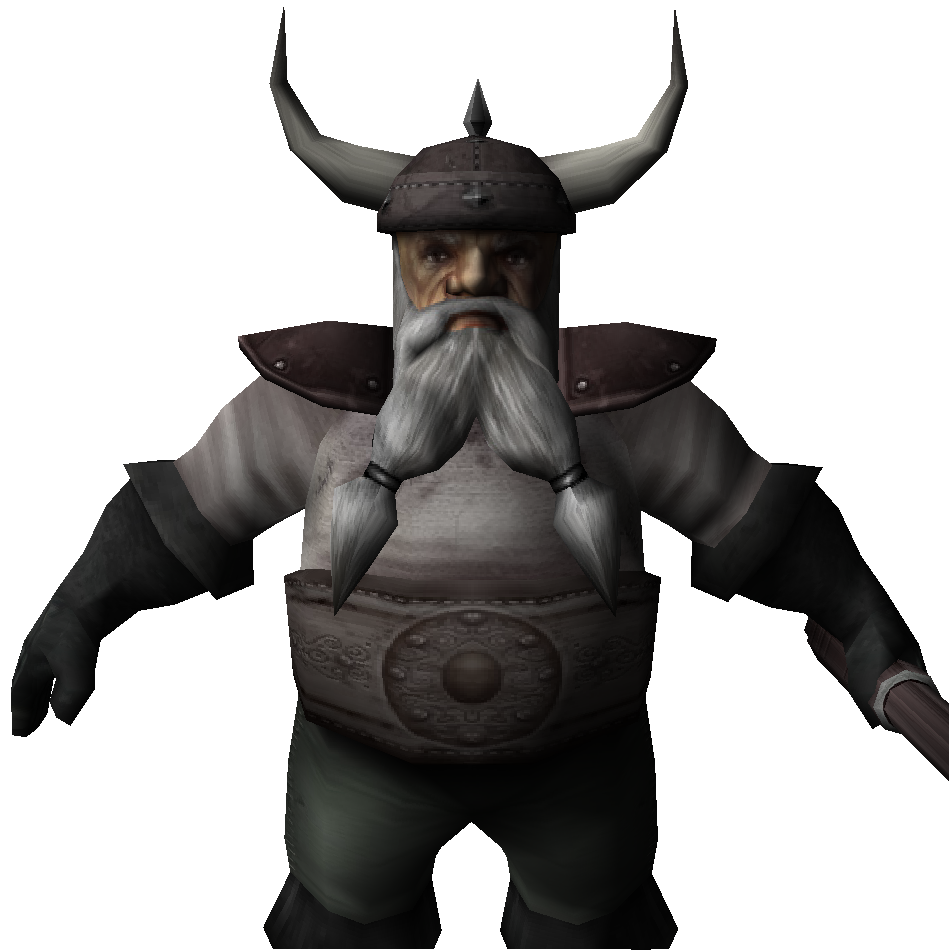
\includegraphics[width=0.39\textwidth]{dwarf_textured}
  \vspace{-10pt}
  \caption{Diffuse Textur kombiniert mit Gouraud Shading.}
  \label{image:modeltextured}
\end{wrapfigure}

Im einfachsten und häufigsten Fall handelt es sich dabei um die Farbe des Objektes (siehe Abbildung \ref{image:modeltextured}). Texturen können aber auch zur Modifikation vieler anderer Parameter eingesetzt werden, beispielsweise als \emph{Alpha Map}, die die Transparenz des Objektes steuert, oder als \emph{Normal Map} für die Flächennormalen, um eine rauhe Oberfläche zu simulieren.

Bei allen Arten von Texturen (mit Ausnahme einiger moderner Verfahren wie \emph{Parallax Occlusion Mapping}, \vglst{parallaxocclusion}{135-154}) muss aber beachtet werden, dass sie die eigentliche Geometrie eines Objektes nicht verändern und damit Vorgänge wie Schatten- und Verdeckungsberechnung nicht beeinflussen. Auch wenn etwa durch eine Normal Map eine strukturierte Oberfläche simuliert wird, erscheint der Rand des Objektes also als gerade Linie, was schnell unrealistisch wirken kann.

\section{Rendering}
\label{rendering}
Beim Rendering wird aus der Beschreibung einer Szene eine zweidimensionale Abbildung, ein \enquote{gerendertes} Bild erzeugt. Zu dieser Beschreibung gehören natürlich die einzelnen Objekte, aber auch Daten über die in der Szene vorhandenen Lichtquellen und die Position des \emph{virtuellen Betrachters}, im Fachjargon auch einfach \emph{Kamera} genannt, \enquote{durch dessen Auge} die Szene betrachtet wird.

Wie oben schon erwähnt, sind grundsätzlich viele Verfahren denkbar, um das Bild zu berechnen. In Anlehnung an die physikalischen Vorgänge in der Realität könnte man zum Beispiel die Photonen, die von den Lichtquellen ausgesendet werden, verfolgen, bis sie absorbiert werden oder auf die virtuelle Kamera treffen. Mit diesem Verfahren wurde tatsächlich unter dem Namen \emph{Photon Tracing} (wörtlich \enquote{Photonenverfolgung}) experimentiert \vglre{wiki:photontracing}. Es erlaubt eine hochrealistische Darstellung der Szene, ist aber für den praktischen Einsatz zu rechenaufwändig, weshalb zu diesem Thema auch kaum wissenschaftliche Publikationen zu finden sind.

Die Idee der Nachverfolung von Strahlen wird von einem anderen Berechnungsverfahren aufgegriffen, dass als \emph{Ray Tracing} (wörtlich \enquote{Strahlverfolgung}) bezeichnet wird. Hier wird aber die Richtung umgekehrt -- statt von den Lichtquelle, wird für jedes Pixel des Bildes ein Strahl von der Kamera emittiert. Wenn dieser Strahl auf ein Objekt trifft, dann werden vom Schnittpunkt neue Strahlen ausgesendet, um Refraktion und Reflexion zu berechnen und zu bestimmen, ob der Punkt von einer Lichtquelle beleuchtet wird oder im Schatten liegt. Da dieses Verfahren je nach Rechenaufwand sehr realistische Ergebnisse liefern kann (beispielweise können Phänomene wie Lichtbrechung optisch korrekt simuliert werden), wird es gerne in Situationen verwendet, in denen mehr Rechenleistung zu Verfügung steht und die Bildqualität wichtig ist, beispielweise für Filme.

Für den Einsatz in Echtzeitsituationen ist aber auch Ray Tracing (derzeit) nicht schnell genug. Deswegen wird auf ein anderes Verfahren zurückgegriffen, das als \emph{Rasterisierung} oder \emph{Scanline Rendering} bezeichnet wird. Dahinter verbirgt sich folgende Idee: Die Abbildung der Szene aus Sicht der virtuellen Kamera kann als Koordinatentransformation aller Objekte in das Koordinatensystem des Bildschirms betrachtet werden. Wenn diese Transformation auf alle Vertices in der Szene angewendet wird, kennt man die Position alle Dreiecke am Bildschirm, man braucht diese also nur noch zu füllen. Dieser Prozess wird als \emph{Rendering-} oder \emph{Grafikpipeline} bezeichnet und wird in der Computergrafik von speziellen Bausteinen übernommen, den Grafikkarten.
% Geschichtliches zu Grafikkarten?

Die Grafikpipeline lässt sich in zwei Abschnitte aufteilen: Zuerst erfolgen die Koordinatentransformationen und einige andere Berechnungen, die auf der Ebene der Eckpunkte ablaufen, sich also der Vektoralgebra bedienen. Danach wird die Farbe der einzelnen Pixel des Ergebnisbildes (das im Normalfall am Bildschirm präsentiert wird) bestimmt, die Berechnungen laufen also auf Pixel-Ebene ab.

In den folgenden beiden Abschnitten werde ich einen Überblick über die Operationen geben, die in der Grafikpipeline stattfinden. Nach einer kurzen Betrachtung der computertechnischen Umsetzung (Abschnitt \ref{hardware}) folgt in Kapitel \ref{3d-transformations} und \ref{viewingtransformations} eine detaillierte Besprechung dieser Operationen aus mathematischer Sicht.


\subsection{Koordinatentransformationen}
\label{coordinatesystems}

\begin{wrapfigure}{R}{0.3\textwidth}
  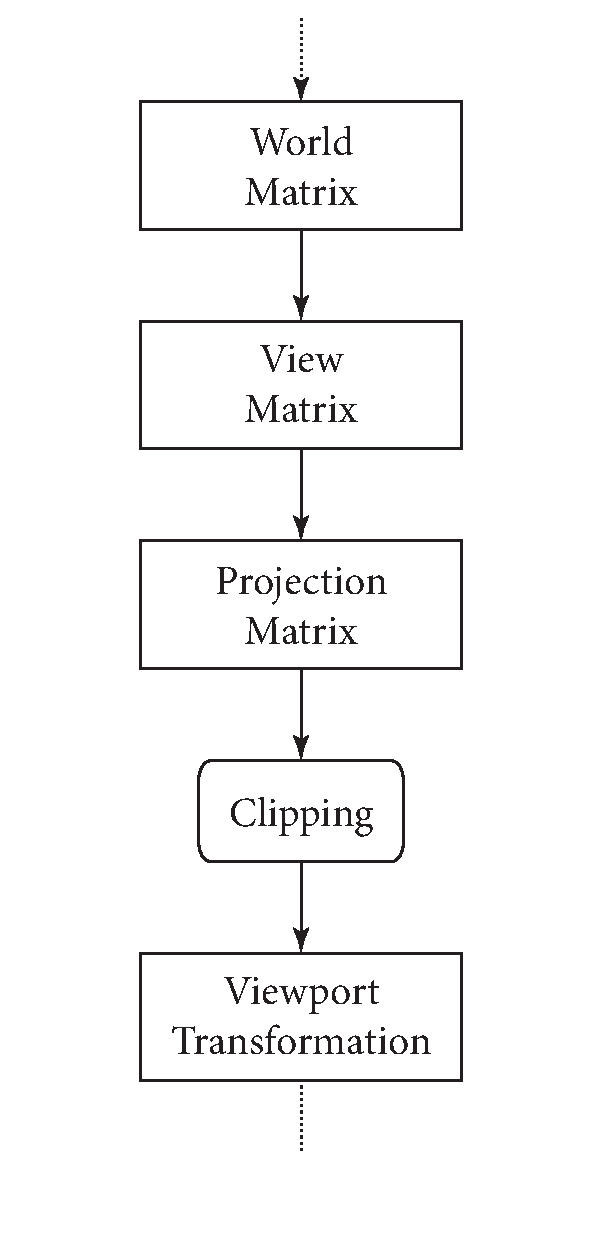
\includegraphics[width=0.29\textwidth]{transformationpipeline}
  \vspace{-10pt}
  \caption{Koordinatentransformationen in der Grafikpipeline.}
\end{wrapfigure}
% @fix: Image (matrix names, other shape for clipping stage)

% Nur karthesische Koordinatensysteme
Wie schon in Abschnitt \ref{vertex} besprochen, wird jeder Körper aus Dreiecken zusammengesetzt, deren Eckpunkte durch Ortsvektoren angegeben werden. Die Koordinaten dieser Vektoren beziehen sich auf das \emph{Modellkoordinatensystem}, das nur für ein Objekt Gültigkeit hat. Ursprung und Einheiten dieses Systems können von dem Künstler, der die Modelle erstellt, im Prinzip beliebig gewählt werden\footnote{In der Praxis wird man natürlich versuchen, sinnvolle Werte zu wählen, also beispielsweise den Ursprung in die Mitte des Objektes legen und eine Einheit als einen Zentimeter interpretieren.}.

Der erste Schritt der Verarbeitung besteht nun darin, die Koordinaten in das \emph{Weltkoordinatensystem} zu übertragen, das eine Bezugsbasis für die gesamte Szene herstellt. Dafür sind normalerweise drei Operationen notwendig, nämlich Translation (um das Objekt an eine bestimmte Stelle zu bewegen), Skalierung (um das Objekt in die richtige Größe zu bringen), und Rotation (um die Ausrichtung des Objekts zu korrigieren). Die Matrix, die diese Transformation beinhaltet, wird \emph{World Matrix} (Weltmatrix) genannt. Im Weltkoordinatensystem sind auch alle anderen Objekte der Szene definiert, etwa die Positionen der Lichtquellen oder der Standpunkt der virtuellen Kamera.

Im nächsten Schritt wird die Szene so transformiert, dass sich die Kamera im Koordinatenursprung befindet und in Richtung der $z$-Achse blickt. Die Matrix, die die Weltkoordinaten in dieses \emph{Kamerakoordinatensystem} transformiert, wird als \emph{View Matrix} (Sichtmatrix) bezeichnet. Sinn dieser Transformation ist es, die nachfolgenden Operationen zu vereinfachen. An dieser Stelle werden auch die Berechnungen ausgeführt, auf die später beim Füllen der Dreiecke zurückgegriffen wird, zum Beispiel Lichtberechnungen auf Vertex-Ebene (mehr dazu in Abschnitt \ref{lighting}).

Als nächstes folgt das \enquote{Herzstück} der 3D-Grafik, die \emph{Projektion} durch die \emph{Projection Matrix}. Diese Operation bildet den gesamten sichtbaren Raum in das \emph{kanonische Sichtvolumen} ab. Dabei handelt es sich um einen mathematisch einfachen Körper, in DirectX (siehe Abschnitt \ref{direct3dopengl}) beispielsweise in einen Quader zwischen den Punkten \textvec{-1}{-1}{0} und \textvec{1}{1}{1}. Diese Abbildung muss zwei Anforderungen erfüllen: Zum einen muss die $x$- und die $y$-Koordinate der Vertices im kanonischen Sichtvolumen schon ihrer endgültigen projizierten Position entsprechen, die projizierte Position muss sich also durch eine einfache orthogonale Parallelprojektion, durch ein \enquote{Weglassen} der $z$-Koordinate ergeben. Zum anderen muss die $z$-Reihenfolge der Vertices erhalten bleiben. Wenn die $z$-Koordinate eines Vektors steigt, muss also auch die $z$-Koordinate des transformierten Vektors (streng monoton) steigen. Dies ist die Voraussetung für die Sichtbarkeits- oder Verdeckungsberechnung, die später stattfindet.

Die Verwendung eines kanonischen Sichtvolumens hat den Vorteil, dass die Art der Projektion keinen Einfluss auf die nachfolgenden Verarbeitungsschritte hat. Unabhängig von der Art der Projektion lassen sich für diese also die gleichen Algorithmen einsetzen, wodurch sich die Umsetzung in Hardware viel effizienter gestalten lässt.

Nach der Projektion werden alle Bereiche verworfen, die sich außerhalb des Sichtvolumens befinden. Dieser Vorgang wird \emph{Clipping} genannt, die Koordinaten nach der Multiplikation mit der Projection Matrix werden daher auch als \emph{Clipping-Koordinaten} bezeichnet.

Um die endgültige Position der Dreiecke zu erhalten, muss das Ergebnis der Projektion nur noch auf die Auflösung des Ausgabemediums \enquote{gestreckt} werden. Dieser Schritt wird als \emph{Viewport Transformation} bezeichnet, die Eckpunkte der Dreiecke liegen danach in \emph{Viewport-Koordinaten} vor. In den meisten Fällen hat dieses Koordinatensystem seinen Ursprung in der linken oberen Ecke des Bildschirms. Die $x$-Koordinaten wachsen dabei nach rechts, die $y$-Koordinaten nach unten.

Unter Anwendung der in Kapitel \ref{transformationmatrixcombination} gezeigten Rechenregel können World, View und Projection Matrix durch Multiplikation leicht in eine Matrix kombiniert werden. Dadurch ist nur mehr eine Matrizenmultiplikation nötig, um einen großen Teil der Transformationen zu erledigen, wodurch dieser Schritt sehr effizient erledigt werden kann.

\subsection{Rasterung}
Nach der Viewport Transformation sind die Koordinatentransformationen abgeschlossen. Nun gilt es, die Dreiecke am Bildschirm zu füllen. Der Speicherbereich, in den die Farbinformationen geschrieben werden, wird als \emph{Framebuffer} bezeichnet.
% @stil: Hinweis auf Computertechnik

Dabei muss darauf geachtet werden, dass Dreiecke, die weiter vom Betrachter entfernt sind (deren $z$-Wert nach der Projektion also größer ist) von den Dreiecken überdeckt werden, die näher beim Betrachter liegen. Dieses sogenannte \emph{Sichtbarkeitsproblem} ist keineswegs so trivial, wie es auf den ersten Blick wirken mag. Zur Lösung dieses Problems hat sich der \emph{Z-Buffer-Algorithmus} durchgesetzt. Dabei wird ein Z-Buffer angelegt, der die gleiche Auflösung wie der Framebuffer hat, zu jedem Pixel des Bildes existiert also ein Wert im Z-Buffer. Zu Beginn der Berechnung werden alle Tiefenwerte auf den größtmöglichen Wert gesetzt, danach werden alle Dreiecke in willkürlicher Reihenfolge gerastert.

Für jedes Pixel wird nun überprüft, ob sein $z$-Wert kleiner ist als der Wert im Buffer, es also näher beim Betrachter ist, als alle vorherigen Pixel. Wenn dies der Fall ist, werden der neue Farbwert und die $z$-Koordinate in den Framebuffer beziehungsweise in den Z-Buffer geschrieben. Andernfalls wird das Pixel verworfen.
% Nachteile des Z-Bufferings, Front-to-Back Rendering

In die Berechnung des Farbwertes der Pixel fließen mehrere Faktoren ein: Die Farbe des Vertices, die Textur(en), die auf das Dreieck angewendet wurden und die Beleuchtung.

\label{lighting}
Die Berechnung der Farbe an einer bestimmten Stelle des Dreieckes ist aus mathematischer Sicht einfach, es muss nur linear zwischen den Farben der Eckpunkte interpoliert werden. Ähnlich verhält es sich auch mit den Texturen -- ausgehend von den Texturkoordinaten der Vertices wird die Stelle interpoliert, an der das Texturbild ausgelesen werden muss. Alle Farbwerte werden miteinander verrechnet und dann mit dem Helligkeitswert multipliziert, den das verwendete Beleuchtungsmodell liefert.

% http://en.wikipedia.org/wiki/Lambert%27s_cosine_law
% Bei allen Interpolationen im Bildschirmkoordinatensystem muss bedacht werden, dass ...
% Extra-Kapitel über Berechnungen auf Pixel-Ebene (perspective-corrected mapping, lighting)?

Nachdem diese Berechnungen für alle Pixel aller sichtbaren Dreiecke durchgeführt worden sind, befindet sich im Framebuffer eine perspektivisch korrekte Abbildung der Szene. Diese muss jetzt nur noch auf dem Bildschirm angezeigt oder in eine Datei geschrieben werden.

\section{Umsetzung in Hardware}
\label{hardware}
So gut wie alle der gerade beschriebenen Berechnungen der Grafik-Pipeline werden in einem modernen Computer von dem Prozessor auf der Grafikkarte erledigt. Der Aufbau dieses Grafikchips ist speziell auf die Pipeline abgestimmt.

Beispielsweise sind eigene optimierte Einheiten für die Transformationen der Vertices zuständig, die auf modernen Grafikkarten durch sogenannte \emph{Vertex Shader} programmiert werden können. Durch die Verwendung von Matrizen lassen sich die meisten Berechnungen auf eine einzige Operation, nämlich die Multiplikation einer Matrix mit einem Vektor, zurückführen. Die Recheneinheiten in der Grafikkarte können nun auf diese Operation ausgelegt werden, wodurch sie sehr schnell arbeiten.

Auch für die Berechnung der Pixelfarben gibt es solche spezielle Einheiten, die durch sogenannte \emph{Fragment-} oder \emph{Pixel-Shader} programmiert werden können. Generell müssen in der Grafikkarte die gleichen Operationen auf eine große Menge Daten angewendet werden. Die Gesamtleistung der Grafikkarte kann also einfach dadurch erhöht werden, dass man viele Einheiten vorsieht, die die Daten parallel abarbeiten\footnote{Die Ende 2008 auf den Markt gekommenen High-End-Modelle der großen Grafikkartenhersteller haben mehrere hundert solcher Einheiten, die parallel arbeiten. \vglr{atispecs,nvidiaspecs}}

\label{direct3dopengl}
Für den Zugriff auf die Grafikkarte haben sich in der Computerprogrammierung zwei große Industriestandards herausgebildet, das von Microsoft entwickelte \emph{DirectX} und das von einem Industriekonsortium rund um den Initiator Silicon Graphics verwaltete \emph{OpenGL}. Die meisten Unterschiede zwischen den beiden Standards sind rein technischer Natur und sind vor dem mathematischen Hintergrund dieser Arbeit nicht weiter relevant.
% @check: Trademarks?

Zwei der Eigenheiten wirken sich aber auch auf die mathematischen Betrachtungen aus. Erstens verwendet DirectX ein linkshändiges, OpenGL aber ein rechtshändiges Koordinatensystem. Bei DirectX führt die $z$-Achse bei wachsender Koordinate also in den Bildschirm hinein, während sie bei OpenGL aus dem Bildschirm herauszeigt. Zweitens, und dieser Punkt hat weitaus größere Auswirkungen, verwendet OpenGL die aus der Schulmathematik bekannten Spaltenvektoren, DirectX aber Zeilenvektoren. Wie schon in Abschnitt \ref{transposition} behandelt, ergibt sich daraus, dass bei einer Kombination mehrerer Transformationen in Matrizenform die Multiplikationsreihenfolge umgekehrt werden muss. Um die Koordinatentransformationen der Grafikpipeline in eine Matrix zusammenfassen, würde man also in OpenGL $M_{ges} = M_{proj} \cdot M_{view} \cdot M_{world}$ rechnen, in DirectX aber $M_{ges} = M_{world} \cdot M_{view} \cdot M_{proj}$. Ich habe mich in dieser Arbeit für die OpenGL-Variante, also rechtshändige Koordinatensysteme und Spaltenvektoren, entschieden, da sie den Konventionen der Schulmathematik entspricht.

\label{performance}
In einem weiteren wichtigen Punkt gleichen sich DirectX und OpenGL wieder sehr: den Techniken, um die Grafikpipeline im Hinblick auf größtmögliche Geschwindigkeit zu optimieren. Die Optimierung kann grundsätzlich auf zwei Ebenen erfolgen: Einerseits versucht man natürlich, die Berechnungen selbst möglichst schnell zu machen. Andererseits versucht man aber auch, unnötige Berechnungen schon von vornherein zu vermeiden.

Unter den ersten Punkt fallen beispielsweise alle Techniken, die den Eigenheiten der Grafikhardware Rechnung tragen. Beispielsweise werden auf einem Computer gewisse Operationen prinzipbedingt sehr schnell ausgeführt, etwa Addition, Subtraktion, und Multiplikation. Andere Operationen sind wesentlich \enquote{teurer} und werden deshalb nach Möglichkeit vermieden. Dazu zählen insbesondere die Division und Operationen wie das Radizieren und die Berechnung transzendenter Funktionen, die der Prozessor annähern muss. Es wird auch versucht, die eingesetzten Algorithmen so zu modifizieren, dass kompliziert zu berechnende Werte nach Möglichkeit zwischengespeichert und mehrfach verwendet werden können.

Der zweite Punkt umfasst alle Techniken, die versuchen, aus der gesamten Menge der Dreiecke schon möglichst bald die Teile auszusortieren, die im fertigen Bild ohnehin nicht sichtbar sind. Beispielsweise könnten in einem Computerspiel, das in einem Bürokomplex spielt, schon von vornherein große Teile der Szene ausgeschlossen werden, weil sie sowieso von den Wänden des Raumes, in dem sich die Kamera gerade befindet, verdeckt werden. Aber auch ohne solche speziellen Annahmen kann typischerweise schon ein großer Teil der Geometrie verworfen werden, bevor er das Ende der Grafikpipeline erreicht. Beispielsweise sind Gegenstände, die sich hinter der Kamera befinden, nie sichtbar und müssen gar nicht erst transformiert werden. Genauso können auch alle von der Kamera abgewandten Polygone eines Objektes verworfen werden, solange das Objekt nicht transparent ist. Die letzgenannte Technik ist unter dem Namen \emph{Backface Culling} bekannt.

Nach diesem kurzen Exkurs auf die computertechnische Seite der 3D-Grafik wenden wir im nächsten Kapitel nun wieder dem mathematischen Teil zu.